\documentclass{article}
\usepackage{graphicx}
\usepackage{circuitikz}
\usepackage{amsmath}
\usepackage{subcaption}
\usepackage{float}

\title{Lab Report: Half-Wave Rectifier Experiment}
\author{ee23BTech11016}
\date{}

\begin{document}

\maketitle

\section*{Aim}
To buid a Half Wave Rectifier

\section*{Apparatus}
\begin{itemize}
    \item AC power supply
    \item Diode 
    \item Resistor (\(R_{\text{load}} = 1 \, \text{k}\Omega\))
    \item Capacitor (\(C_{\text{filter}} = 1 \, \mu F\)) [Filter]
    \item Oscilloscope
    \item Multimeter
    \item Connecting wires
\end{itemize}

\section*{Circuit Diagrams}
\begin{figure}[h]
    \centering
    \begin{subfigure}{0.45\textwidth}
        \centering
        \begin{circuitikz}
  \draw (0,0)
  to[V, v<=\(V_{\text{in}}\)] (0,2)
  to[Do, v<=\(V_{\text{out}}\)] (2,2)
  to[R, l=\(R_{\text{load}}\)] (2,0)
  -- (0,0);
  \draw (2,2) -- (3,2) node[right] {\(V_{\text{out}}\)};
        \end{circuitikz}
        \caption{With Filter Capacitor}
        \label{fig:circuit_with_filter}
    \end{subfigure}
    \begin{subfigure}{0.45\textwidth}
        \centering
        \begin{circuitikz}
  \draw (0,0)
  to[V, v<=\(V_{\text{in}}\)] (0,2)
  to[Do, v<=\(V_{\text{out}}\)] (2,2)
  to[C, l=\(C_{\text{filter}}\), v>=\(V_{\text{c}}\)] (2,0)
  -- (0,0);
  \draw (2,2) -- (4,2)
  to[R, l=\(R_{\text{load}}\)] (4,0)
  -- (2,0);
        \end{circuitikz}
        \caption{Without Filter Capacitor}
        \label{fig:circuit_without_filter}
    \end{subfigure}
    \caption{Half-Wave Rectifier Circuit Diagrams}
    \label{fig:circuit_diagrams}
\end{figure}

\section*{Theory}
\begin{enumerate}
\item A half-wave rectifier is a simple electronic circuit that converts alternating current (AC) to direct current (DC).
\item The basic principle behind a half-wave rectifier is to allow only one half-cycle of the AC waveform to pass through, resulting in a pulsating DC output.
\item During the positive half-cycle of the AC input voltage, the diode conducts and allows current to flow through the load. 
\item However, during the negative half-cycle, the diode blocks the current, resulting in no output.
\end{enumerate}

\section*{Procedure}
\begin{enumerate}
    \item Set up the circuit as shown in Figure \ref{fig:circuit_with_filter} or Figure \ref{fig:circuit_without_filter}.
    \item Connect the oscilloscope to measure the input and output waveforms.
    \item Gradually increase the AC voltage and record the readings.
    \item Measure the output DC voltage and ripple using a multimeter.
\end{enumerate}

\section*{Calculation}

\subsection*{Output Voltage Calculation}

The output voltage (\(V_{\text{out}}\)) of the half-wave rectifier can be calculated using the formula mentioned in the theory section:

\begin{align}
V_{\text{out}} &= V_{\text{max}} \cdot \frac{T}{2\pi} \cdot \left(1 - \cos\left(\frac{2\pi t}{T}\right)\right) \nonumber\\ 
&= \nonumber \\
&=
\end{align}

Where:
\begin{align*}
    V_{\text{max}} & : \text{Peak value of the AC input voltage} \\
    T & : \text{Period of the AC input waveform} \\
    t & : \text{Time}
\end{align*}

\subsection*{Average Output Voltage}

The average output voltage (\(V_{\text{avg}}\)) can be calculated by integrating \(V_{\text{out}}\) over one complete cycle and dividing by the period \(T\):

\begin{align}
V_{\text{avg}} &= \frac{1}{T} \int_{0}^{T} V_{\text{out}} \, dt \nonumber\\ 
&= \nonumber \\
&=
\end{align}

[Include the integration steps and final result.]

\subsection*{Ripple Factor}

The ripple factor (\(\gamma\)) is a measure of the AC component in the rectified output and can be calculated using the formula:

\begin{align}
\gamma &= \frac{\sqrt{\frac{1}{T} \int_{0}^{T} (V_{\text{out}} - V_{\text{avg}})^2 \, dt}}{V_{\text{avg}}} \nonumber\\ 
&= \nonumber \\
&= 
\end{align}

\section*{Observations}
During the experiment, the following observations were made:

\begin{enumerate}
    \item \textbf{Input Voltage (\(V_{\text{in}}\)):} 

    \item \textbf{Output Voltage (\(V_{\text{out}}\)):} 

    \item \textbf{Ripple Voltage:} 

    \item \textbf{Filter Capacitor Voltage (\(V_{\text{c}}\)):} 

    \item \textbf{Load Resistor Voltage (\(V_{\text{load}}\)):} 

   
\end{enumerate}

\section*{Lab Status}
\begin{figure}[H]
    \centering
    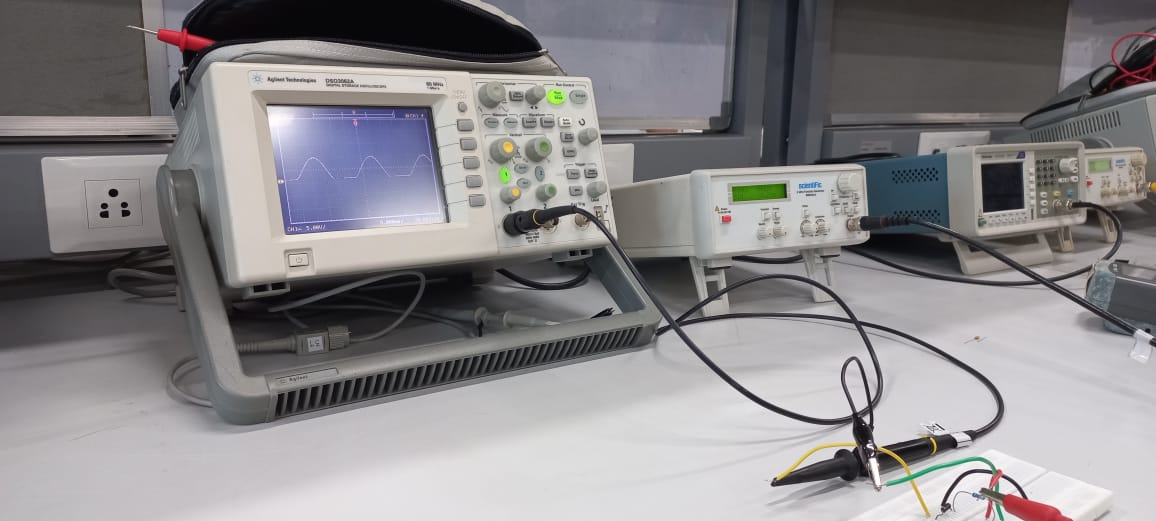
\includegraphics[width=0.8\textwidth]{fig.jpeg}
\end{figure}


\section*{Conclusion}
In conclusion, the half-wave rectifier is a fundamental circuit for converting AC to DC. While simple and cost-effective, its limitations in efficiency and output quality make it suitable for specific low-power applications
\end{document}

